%*********************************************************************
%	CHAPTER 4 - SYSTEM DESIGN AND IMPLEMENTATION
%*********************************************************************
% PURPOSE OF THIS CHAPTER
%   Everything that was BUILT and then held FIXED across the experiments:
%   hardware, test environment, software, what each pipeline stage does,
%   and how accuracy is measured.
%
% WHERE THINGS GO (rule of thumb)
%   - Choice justified by a datasheet or a calculation (e.g. tag size from
%     the pinhole model)  -> explain it HERE.
%   - Choice made by running a test (filter sweep, detector tuning,
%     compensation method, depth matcher, pose method, fusion method)
%     -> only LIST the candidates here and point forward with
%        "selected in Section~\ref{...}". The test itself lives in Ch5 / 5b.
%
% CROSS-REFERENCES
%   Ch3 = theory (why it works). Ch4 = implementation (how it was done here).
%   Avoid rederiving equations from Ch3; cite the Ch3 section instead.
%*********************************************************************
\chapter{Methodology}
\label{ch:design}

\section{System Description}
%---------------------------------------------------------------------
This chapter describes the system and data used in this project.
\autoref{sec:ch4.hardware} describes the underwater \gls{rov} used for data collection, and \autoref{sec:ch4.laptop} the processing laptop.
\autoref{sec:ch4.software} gives an overview of the processing pipeline and software used.
\autoref{sec:testplatform} describes the calibration board and test rig built for this project, \autoref{sec:ch4.targets} the test targets,
and \autoref{sec:ch4.datasets} the datasets recorded with them.

%=====================================================================
% 1) DESIGN REQUIREMENTS
%    Turn the project objectives (Ch1, sec "Project objectives") into
%    numbers that later sections design against. A small table works well:
%      Requirement            | Value               | Source / reason
%      Working range          | 0.3 - 2.0 m         | min focus 25 cm; scan distance under ice
%      Worst-case turbidity   | ~3 NTU              | bloom turbidity spikes (Garcia 2020, Schallenberg 2019)
%      Min tag size in image  | >= 40 px            | underwater detection margin (see boardsizing)
%      Image resolution       | 1600 x 1200         | sensor max
%      Accuracy target        | ?? mm               | TODO: decide - what accuracy is "useful" for ice draft?
%    Each later design choice should point back to one of these rows.

% 2) PIPELINE BLOCK DIAGRAM
%    Implementation version of fig:ch3.pipeline - do NOT redraw the theory
%    figure. Each block gets the script/module that does it:
%
%      Video (.mp4, L+R)
%        -> Frame extraction ............. preproccessing/extract_stereo_frames.py,
%                                          blur_check.py, select_scan_frames.py
%        -> Channel selection + filtering  experiments/channels/
%        -> Tag detection + calibration .. 01_Calibration/Calibration.py,
%                                          detector_presets.json
%        -> Refraction compensation ...... experiments/compensation/
%        -> Rectify + depth per frame .... 03_Reconstruction/depth_frames.py,
%                                          dense_stereo.py (SGBM / FoundationStereo / AquaStereo)
%        -> Pose per frame ............... tag_poses.py / icp_poses.py / colmap_poses.py
%        -> Fusion ....................... tsdf_fuse.py / median_fuse.py / colmap_mvs.py
%        -> Evaluation ................... 04_Comparison/compare_to_cad.py, score_objects.py
%
%    Note the split after frame extraction: filtering for DETECTION is not
%    the same as filtering for 3D RECONSTRUCTION (old note:
%    "Filtering (for detection) -> detection" vs "Filtering (for 3D recon)
%    -> Compensation -> 3D reconstruction"). Show this as two branches.
%    TODO: draw in draw.io (diagram style rules), export PDF to fi tgs/Ch4/.
%
% \begin{figure}[H]
%     \centering
%     \includegraphics[width=\textwidth]{figs/Ch4/pipeline_impl.pdf}
%     \caption[Implemented pipeline]{\textbf{Implemented pipeline.} Each block
%     is labelled with the script that performs it. Stages with several
%     candidate methods are compared in Chapters~\ref{ch:experiments} and 5b.}
%     \label{fig:ch4.pipeline}
% \end{figure}


%=====================================================================
\subsection{Hardware}
\label{sec:ch4.hardware}
%=====================================================================
% Order: cameras -> how they are mounted -> lighting -> calibration target.
 
This project uses a BlueROV2 Heavy, a low-cost underwater \gls{rov} for research and inspection made by Blue Robotics
\cite{bluerobBlueROV2}. The standard configuration has six thrusters. The Heavy configuration adds two more,
giving the \gls{rov} active roll and pitch control  \cite{bluerobBlueROV2Heavy}.
 
In addition to the vehicle's standard forward monocular camera,
two \gls{dwe} StellarHD cameras \cite{dweStellarHDDatasheet} are fitted in a stereo camera configuration, 
with a 150\,mm baseline. Both have Aquagon lenses \cite{dweAquagon} and are mounted to the lower front of the frame.
Four Lumen subsea lights at the front of the \gls{rov} provide adjustable lighting
 \cite{bluerobLumen}.

 \begin{figure}[H]
    \centering
    \begin{tikzpicture}[
    callout/.style={draw=black!80, fill=black!4, font=\footnotesize, align=center,
                    minimum width=3cm, minimum height=0.6cm, inner sep=2pt, anchor=west},
    pointer/.style={draw=rovblue, line width=1pt, -{Latex[length=2.2mm]}},
    trunk/.style={draw=rovblue, line width=1pt}]
  \definecolor{rovblue}{HTML}{1A73E8}
  \definecolor{rovred}{HTML}{E53935}
  \node[anchor=south west, inner sep=0] (img) at (0,0)
    {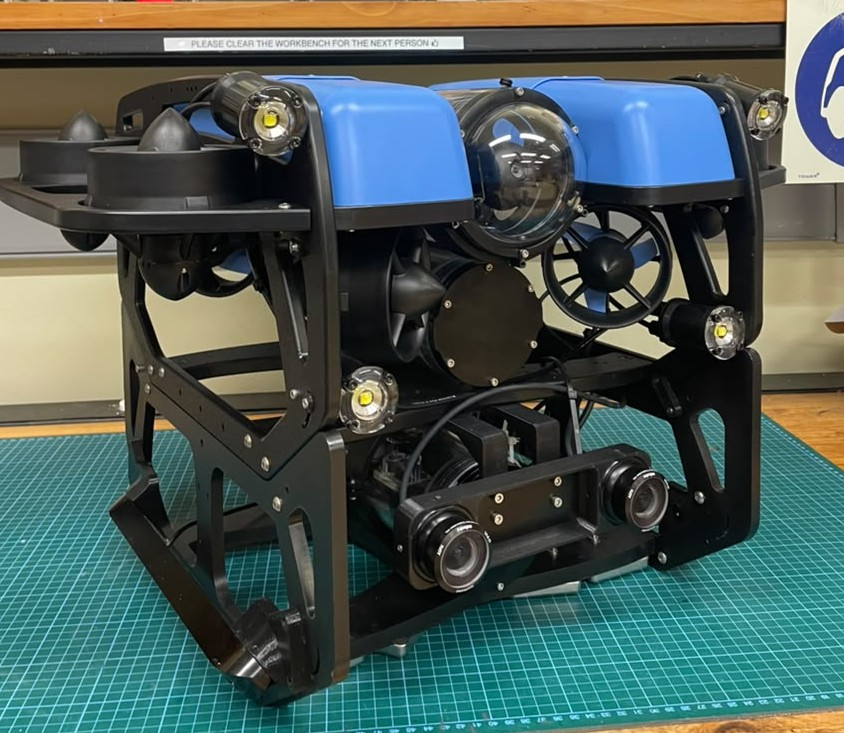
\includegraphics[width=0.40\textwidth]{figs/Ch4/Rovyn.jpeg}};
  \begin{scope}[x={(img.south east)}, y={(img.north west)}]
    % Positions as fractions of the photo (0,0 bottom left; 1,1 top right)
    \coordinate (camL) at (0.547, 0.240);
    \coordinate (camR) at (0.764, 0.318);
    \coordinate (lt1)  at (0.320, 0.836);
    \coordinate (lt2)  at (0.906, 0.843);
    \coordinate (lt3)  at (0.855, 0.550);
    \coordinate (lt4)  at (0.432, 0.457);
    \def\tx{1.03}
    % Labels
    \node[callout, minimum height=0.9cm] (lights) at (1.07, 0.62)
      {4\,$\times$ \href{https://bluerobotics.com/store/thrusters/lights/lumen-r2-rp/}{\textcolor{blue}{Blue Robotics Lumen}}\\
       lights, 1500\,lm, 135$^\circ$ beam};
    \node[callout, draw=rovred, fill=white, text=rovred] (base) at (1.07, 0.44) {Baseline 150\,mm};
    \node[callout, minimum height=0.9cm] (cams) at (1.07, 0.27)
      {2\,$\times$ \href{https://dwe.ai/products/stellarhd}{\textcolor{blue}{DWE StellarHD}}\\
       stereo cameras};
    % Lights: one trunk, four branches
    \draw[trunk] (lights.west) -- (\tx, 0.62);
    \draw[trunk] (\tx, 0.93) -- (\tx, 0.457);
    \draw[pointer] (\tx, 0.843) -- ($(lt2)+(0.035,0)$);
    \draw[pointer] (\tx, 0.550) -- ($(lt3)+(0.035,0)$);
    \draw[pointer] (\tx, 0.457) -- ($(lt4)+(0.035,0)$);
    \draw[pointer] (\tx, 0.93) -- (0.320, 0.93) -- ($(lt1)+(0,0.035)$);
    % Cameras
    \draw[pointer] (cams.west |- camR) -- ($(camR)+(0.045,0)$);
    \draw[pointer] (cams.west |- camL) -- ($(camL)+(0.03,0)$);
    % Baseline
    \draw[rovred, line width=1.2pt, {Latex[length=2.2mm]}-{Latex[length=2.2mm]}] (camL) -- (camR);
    \coordinate (mid) at ($(camL)!0.5!(camR)$);
    \draw[rovred, line width=1pt] (base.west) -| (mid);
    \fill[rovred] (mid) circle (1.6pt);
  \end{scope}
\end{tikzpicture}

    \caption[Stereo camera rig]{\textbf{Stereo camera platform.} The two StellarHD
    cameras and four Lumen lights mounted on the BlueROV2, with the 150\,mm baseline marked.}
    \label{fig:ch4.rig}
\end{figure}
 
The vehicle is controlled by a \gls{rpi} with a
Blue Robotics Navigator flight controller \cite{bluerobNavigator}. The Navigator is an \gls{rpi}
expansion board that provides the \gls{imu}, compass,
barometer, \gls{adc} and \gls{pwm} outputs for the thrusters and lights
\cite{bluerobNavigator}. A \gls{dvl}, side scanning sonar, and the three cameras are connected over USB and Ethernet ports.
% TODO: confirm models (e.g. Ping360 is a *mechanical scanning* sonar, not side-scan).
%---------------------------------------------------------------------
\subsubsection{Cameras and lenses}
\label{subsec:ch4.cameras}
%---------------------------------------------------------------------
% Sources:
% https://storage.googleapis.com/docs-product-files/stellarHD-series/stellarHD/datasheets/stellarHD-datasheet.pdf
% One of these; https://www.ovt.com/products/#image-sensor?is_technology=omnipixel3-gs
% TODO: cite the datasheets in the caption / text (add to Zotero, not the .bib).
% TODO: explain how the lenses are optically corrected, giving a different
%       FOV in air and in water (links to Ch3 "Calibrating underwater").
The StellarHD cameras are fitted with \gls{dwe}'s Aquagon lenses, which are designed to counteract the effects of the underwater environment
by correcting for distortion and chromatic aberration \cite{dweAquagon}.
A flat port refracts light, narrowing the field of view and distorting the image
(\autoref{subsec:ch3.underwater_calib}). Corrective optics address this by placing additional lens elements behind the port, so that the camera sees an undistorted
virtual image equivalent to the scene in air \cite{slaterAfocalViewportOptics2014}.
The Aquagon lenses have seven elements, two aspherical and two \gls{ed}.
These are fitted behind a sapphire front port. The manufacturer quotes distortion below 1.5\,\% in water \cite{dweStellarHDDatasheet}.
The key camera specifications are listed in \autoref{table:ch4.cameraspecs}.
% Bullet lists from the old draft merged into one table.
\begin{table}[H]
    \centering
    \caption[Camera and lens specifications]{\textbf{Camera and lens specifications} \cite{dweStellarHDDatasheet}.}
    \label{table:ch4.cameraspecs}
    \renewcommand{\arraystretch}{1.35}
    % No gaps in the vertical rule where it meets the horizontal ones
    \setlength{\aboverulesep}{0pt}
    \setlength{\belowrulesep}{0pt}
    \begin{tabularx}{\textwidth}{@{} l X | l X @{}}
    \toprule[2.25pt]
    \multicolumn{2}{@{}l|}{\textbf{StellarHD sensor}} & \multicolumn{2}{l@{}}{\textbf{Aquagon lens}} \\
    \midrule[1pt]
    Sensor        & 1/2.9-inch OmniPixel3-GS \acrshort{cmos} & Focus          & Fixed \\
    Pixel size    & 3 $\times$ 3\,\textmu m        & Focal length   & 3.0\,mm \\
    Shutter       & Global                         & Aperture       & f/1.6 \\
    Resolution    & 1600 $\times$ 1200             & Min.\ focus    & 25\,cm \\
    Frame rate    & Up to 60\,fps (\acrshort{mjpeg})          & Distortion     & $< 1.5$\,\% \\ % TODO: measured how?
                  &                                & \acrshort{fov}$^{*}$ (H/V/D) & 78\textdegree{}/67\textdegree{}/93\textdegree{} \\
    \bottomrule[2.25pt]
    \end{tabularx}
    \par\smallskip
    {\footnotesize\raggedright $^{*}$Value for the Aquagon lens's field of view in water.\par}
\end{table}

The StellarHD cameras support leader follower frame synchronisation, 
however, the current setup does not have the required shared cabling.
This frame synchronisation is only 
supported at 60\,fps, limiting it to \gls{mjpeg}\footnote{Video stored as a sequence of individually JPEG-compressed frames.} recordings.
In the current configuration, the two cameras can start with a time offset
and drift apart during a recording.

\subsection{Control and processing laptop} 
\label{sec:ch4.laptop}
The BlueROV2 connects to a laptop through its tether and a tether interface
adapter \cite{bluerobFXTI}. The laptop runs Blue Robotics' Cockpit software \cite{bluerobCockpit}, and the \gls{rov} is piloted
with an Xbox controller. The same laptop was used for all post-processing in this project.
Its specifications are listed in \autoref{table:ch4.laptopspecs}.

\begin{table}[H]
    \centering
    \caption[Control and processing laptop specifications]{\textbf{Control and processing laptop specifications} \cite{lenovoLOQ15IRX10}.}
    \label{table:ch4.laptopspecs}
    \renewcommand{\arraystretch}{1.35}
    \begin{tabular}{@{} l l @{}}
    \toprule[2.25pt]
    \textbf{Component} & \textbf{Specification} \\
    \midrule[1pt]
    Model            & Lenovo LOQ 15IRX10 \\
    Operating system & Ubuntu 26.04 LTS \\
    \acrshort{cpu}   & Intel Core i7-14700HX \\
    \acrshort{gpu}   & NVIDIA GeForce RTX 5060 Laptop, 8\,GB \acrshort{vram} \\
    Memory           & 32\,GB DDR5 \acrshort{ram} \\
    \bottomrule[2.25pt]
    \end{tabular}
\end{table}

%=====================================================================
\subsection{Software}
\label{sec:ch4.software}
%=====================================================================
% Keep short: a table plus one paragraph on code layout and config.
% Versions taken from src/requirements.txt and src/venv on 2026-10-22.
% CHECK: Open3D is in requirements.txt but not installed in src/venv -
%        confirm which environment the TSDF runs used.
% CHECK: COLMAP version (4.3 mentioned in code comments) and the
%        FoundationStereo / AquaStereo checkpoints + PyTorch/CUDA version.
The software used in this project is split into two parts: the camera control and recording software that runs on the \gls{rov}
(\autoref{subsec:ch4.recording}), and the Python pipeline that processes the recordings on the laptop (\autoref{subsec:ch4.postprocessing}).
\subsection{Camera control and recording}
\label{subsec:ch4.recording}
A custom Python script (\texttt{stereo\_cam.py}) controls both StellarHD 
cameras through the Video4Linux2 (V4L2) API \cite{linuxV4L2}. 
It configures resolution, frame rate, pixel format, exposure,
 white balance and image controls.

Recording saves the cameras' raw \gls{mjpeg} or YUYV\footnote{YUYV: an uncompressed format that stores brightness for every pixel and colour for every pair of pixels.} frames to the Pi's \gls{sd} card or an 
external \gls{ssd}. In parallel, both feeds are transcoded to H.264 and streamed 
over the tether to a MediaMTX server, letting the operator view the live stereo 
feed in a browser during data collection. Each recording produces one video file per camera (\texttt{left.mkv} and \texttt{right.mkv}) and a
\gls{csv} file per camera recording the capture time of every frame (\texttt{left\_timestamps.csv} and \texttt{right\_timestamps.csv}).
These timestamps are later used to pair each right frame with its closest left frame. The timestamps are used to check for large
timing offsets between the two cameras.


\subsubsection{Post-processing software}
\label{subsec:ch4.postprocessing}
The code base is split into four pipeline stages. Each stage is a standalone script, 
which utilises the previous stages' outputs as an input. This allows stages to be swapped out and compared without
rerunning the earlier stages. Each experiment is defined by a \acrshort{json} configuration file that states every
setting. Each stage saves its output in a standard
format, such as YAML for camera calibrations. Each run 
writes a manifest file recording the configuration and code version that
produced the results. For the folder structure, file formats and instructions on running the code,
refer to the project's
\href{https://github.com/GlenOJones/UCT_Final_Year_Project}{\textcolor{blue}{GitHub repository}}.

 \begin{figure}[htbp]
    \centering
    % Font: TeX Gyre Heros (Helvetica clone) on XeLaTeX, \sffamily on pdfLaTeX.
    \ifdefined\newfontfamily
        \ifdefined\pipelinefont\else
            \newfontfamily\pipelinefont{texgyreheros}[Extension=.otf, UprightFont=*-regular, BoldFont=*-bold]
        \fi
    \else
        \providecommand{\pipelinefont}{\sffamily}
    \fi
    \begin{tikzpicture}[font=\pipelinefont\fontsize{8}{9.6}\selectfont,
      box/.style={draw=black, line width=0.4pt, align=center, minimum height=16mm, inner sep=0.6mm},
      ends/.style={draw=black, rounded corners=2mm, line width=0.4pt, align=center, minimum height=16mm, inner sep=1mm},
      stage/.style={font=\pipelinefont\fontsize{8}{9.6}\selectfont\bfseries, text height=1.6ex, text depth=0.4ex},
      flow/.style={-{Stealth[length=2mm]}, line width=0.4pt}]
      \node[ends, minimum width=14mm, text width=12.8mm] (n0) at (7.0mm,0) {Stereo\\recording};
      \node[box, minimum width=21mm, text width=19.8mm] (n1) at (27.5mm,0) {extract\_stereo\_\\frames.py\\(GUI)};
      \node[stage, above=1.2mm of n1] {Frame extraction};
      \node[box, minimum width=20mm, text width=18.8mm] (n2) at (51.0mm,0) {Calibration.py};
      \node[stage, above=1.2mm of n2] {Calibration};
      \node[box, minimum width=15mm, text width=13.8mm] (n3) at (71.5mm,0) {depth\_\\frames.py};
      \node[stage, above=1.2mm of n3] {Depth};
      \node[box, minimum width=23mm, text width=21.8mm] (n4) at (93.5mm,0) {tag\_poses.py\\colmap\_poses.py\\icp\_poses.py};
      \node[stage, above=1.2mm of n4] {Pose};
      \node[box, minimum width=21mm, text width=19.8mm] (n5) at (118.5mm,0) {tsdf\_fuse.py\\colmap\_mvs.py};
      \node[stage, above=1.2mm of n5] {Fusion};
      \node[box, minimum width=19mm, text width=17.8mm] (n6) at (141.5mm,0) {postprocess\_\\cloud.py};
      \node[stage, above=1.2mm of n6] {Clean-up};
      \node[ends, minimum width=11mm, text width=9.8mm] (n7) at (159.5mm,0) {Point\\cloud};
      \foreach \a/\b in {n0/n1, n1/n2, n2/n3, n3/n4, n4/n5, n5/n6, n6/n7}
          \draw[flow] (\a) -- (\b); % NOTE (moved out of the TikZ code): want the first section named
    \end{tikzpicture}
    \caption[Processing pipeline]{\textbf{Processing pipeline.} The stages from a stereo recording to a fused point cloud, each labelled with the script that runs it. Where a stage lists several scripts, these are alternative methods that are compared in later chapters.}
    \label{fig:ch4.pipeline}
\end{figure}

The versions of the libraries and tools used are listed in the appendix (\autoref{app:software}).

%=====================================================================
% SECTION: Dataset (moved from 4b_dataset.tex)
%=====================================================================
\section{Calibration Board and Test Platform Construction}
\label{sec:testplatform}

%=====================================================================
% SECTION: Test rig and Dataset
%=====================================================================
This project produced not only a report, but also an in-air and underwater
stereo dataset. The dataset contains calibration recordings of an AprilGrid
board \cite{furgaleUnifiedTemporalSpatial2013}, side scans of 3D-printed shapes with known \gls{cad} geometry, and
upward-looking scans of foam blocks that imitate the underside of sea ice.
This chapter first describes the calibration board and the sliding test rig used
to collect the data, then the reconstruction targets, and finally the three
datasets (DS1 to DS3) and the conditions they were recorded in.
%==============
\subsection{Calibration Board and test Rig Construction}


% Calibration board
As explained in \autoref{subsec:ch3.targets}, an AprilGrid can still be used for
calibration when only some of its tags are detected. To get a target that is flat and
waterproof, a custom AprilGrid was generated with Kalibr
\cite{furgaleUnifiedTemporalSpatial2013, kalibrRepo} and printed on white aluminium
Dibond (\href{https://www.ormsprintroom.co.za/product/metal-prints/}{\textcolor{blue}{Orms Print Room}}, Cape Town). The board was sized as A1 with 35.36\,mm
tags.

A custom sliding rig was built from 2020 aluminium extrusion. The \gls{rov} is
secured to 3D-printed rollers with ball bearings, which run along the
horizontal extrusions. This lets it slide towards and away from the calibration
board at the end of the rail. The board sits on an adjustable mount with two settings.
Its tilt can be set from horizontal to vertical in 10\,$^\circ$ steps, and the mount can be
positioned at the left, centre or right of the rail's end. This gives a repeatable distance, position
and angle between the board and the cameras across tests. The \gls{cad} files
for the sliding rail and calibration board image can be found in the project's
\href{https://github.com/GlenOJones/UCT_Final_Year_Project/tree/main/CAD}{\textcolor{blue}{GitHub repository}}.

\begin{figure}[htbp]
    \centering
    % Both photos are 4:3, so equal widths give identical sizes
    \begin{subfigure}[t]{0.48\textwidth}
        \centering
        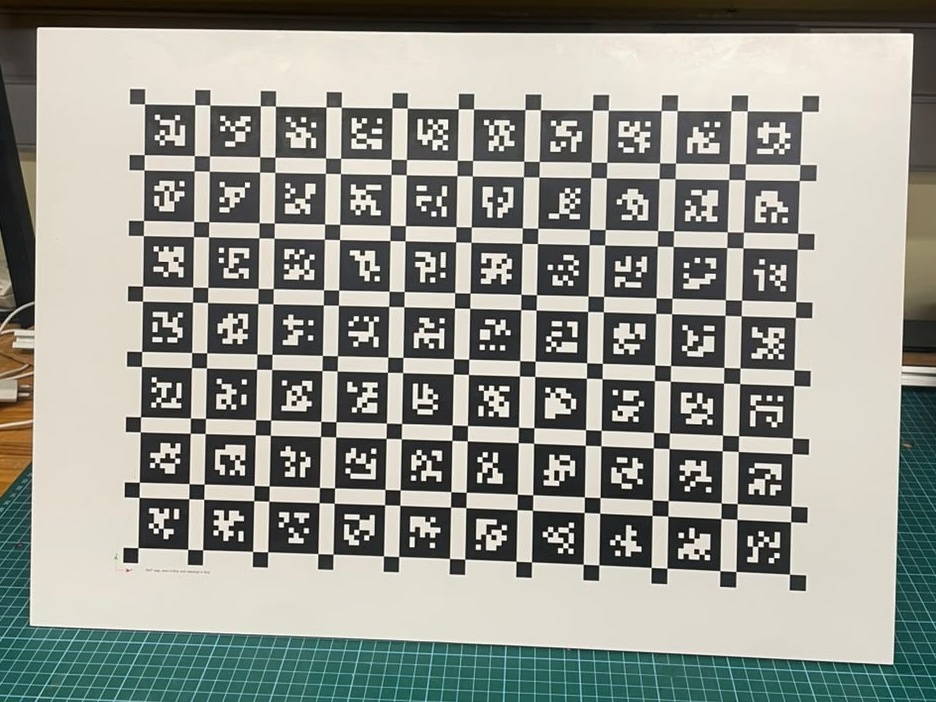
\includegraphics[width=\linewidth]{figs/Ch4/Board.jpeg}
        \caption{Calibration board.}
        \label{fig:ch5.board}
    \end{subfigure}
    \hfill
    \begin{subfigure}[t]{0.48\textwidth}
        \centering
        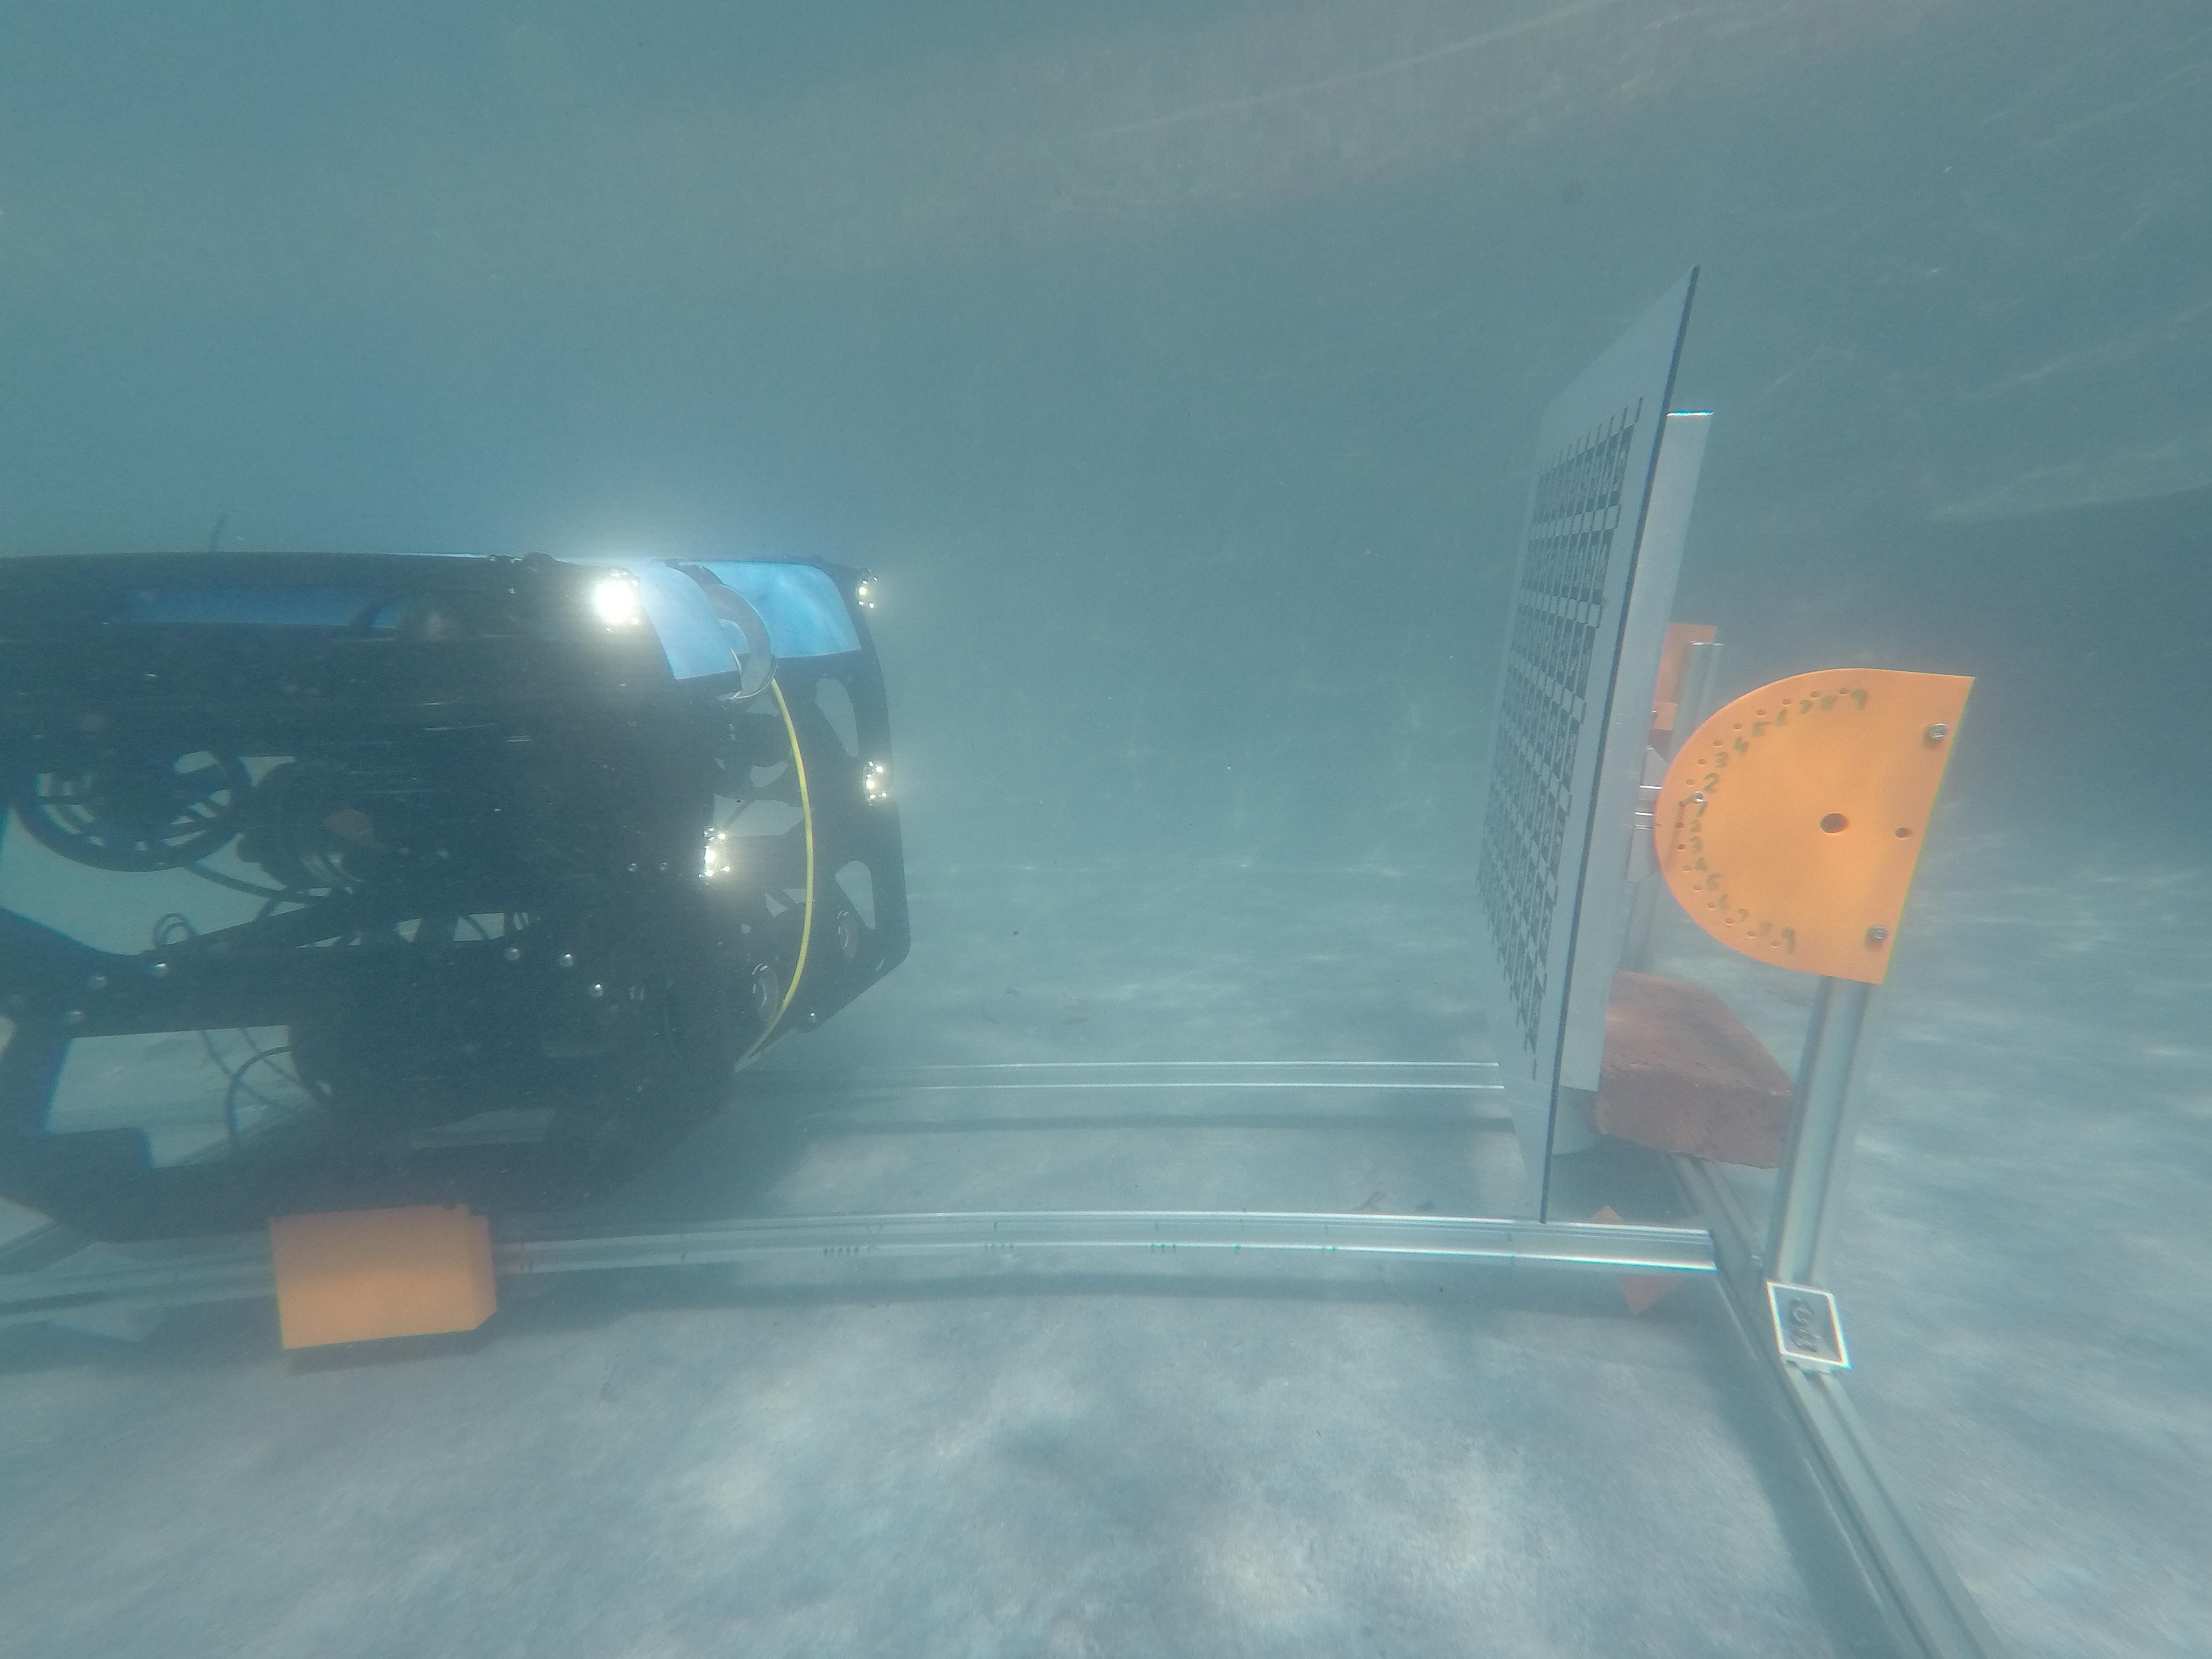
\includegraphics[width=\linewidth]{figs/Ch5/Rig_In_Water.jpeg}
        \caption{Sliding rig underwater.}
        \label{fig:ch5.rig_in_water}
    \end{subfigure}
    \caption[Calibration board and sliding test rig]{\textbf{Calibration board and sliding test rig.}
    (a) The AprilGrid board: 10\,$\times$\,7 AprilTag 36h11 tags (35.36\,mm tags, 10.61\,mm gaps) on aluminium Dibond.
    (b) The rig underwater: the \acrshort{rov} slides along the rail towards the board, which can be tilted in 10\,$^\circ$ steps.
    The board appears curved only because of the GoPro's wide-angle lens; it is flat.}
    \label{fig:ch5.test_rig}
\end{figure}

%==================

\section{Test Targets}
\label{sec:ch4.targets}
Two sets of targets were scanned to test the pipeline. 3D-printed shapes with known geometry are used to measure
reconstruction accuracy, while painted foam structures provide a closer approximation of the ice underside.

\subsection{3D-printed targets}
\label{subsec:ch5.3d_printed_shapes}
The 3D-printed targets were designed by Agoritsa Spirakis for a \acrshort{uct}
project \cite{aggi_thesis}. The set used here contains two pyramid
tiles and two sinusoidal tiles.
\autoref{fig:ch5.printed_shapes} shows the four shapes and \autoref{fig:ch4.data_side} depicts these during data collection,
described in \hyperref[sec:ch4.ds2]{Section~\ref*{sec:ch4.ds2}}. 
These targets act as a ground truth as their exact geometries are known. The reconstructed
point clouds are compared against them to measure accuracy.


% TODO: create the appendix with the shape images and add \label{app:printed_shapes}

\begin{figure}[htbp]
    \centering
    \begin{subfigure}[b]{0.24\textwidth}
        \centering
        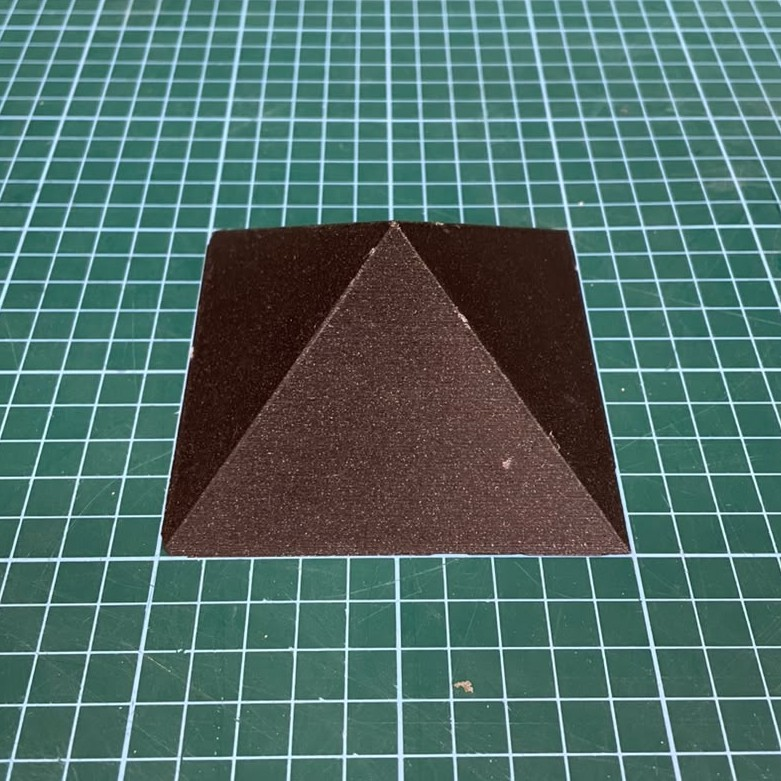
\includegraphics[width=\linewidth]{figs/Ch4/1_pyr.jpeg}
        \caption{Pyramid}
        \label{fig:ch5.print_pyramid}
    \end{subfigure}
    \hfill
    \begin{subfigure}[b]{0.24\textwidth}
        \centering
        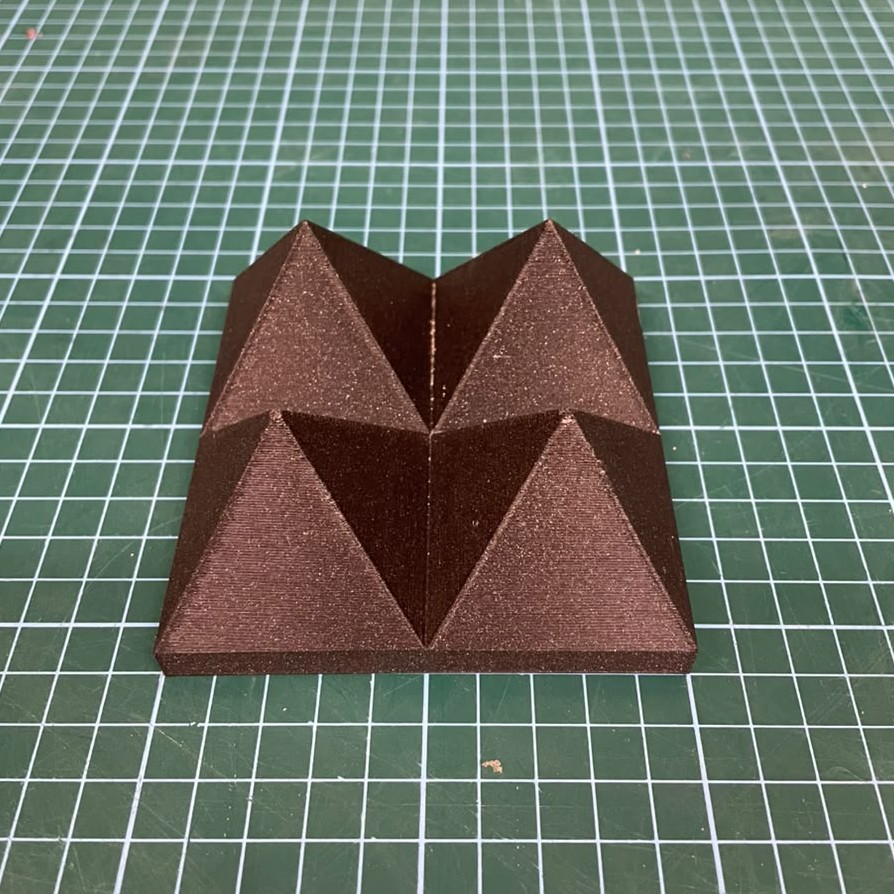
\includegraphics[width=\linewidth]{figs/Ch4/2_pyr.jpeg}
        \caption{Pyramid 2\,$\times$\,2}
        \label{fig:ch5.print_pyramid_2x2}
    \end{subfigure}
    \hfill
    \begin{subfigure}[b]{0.24\textwidth}
        \centering
        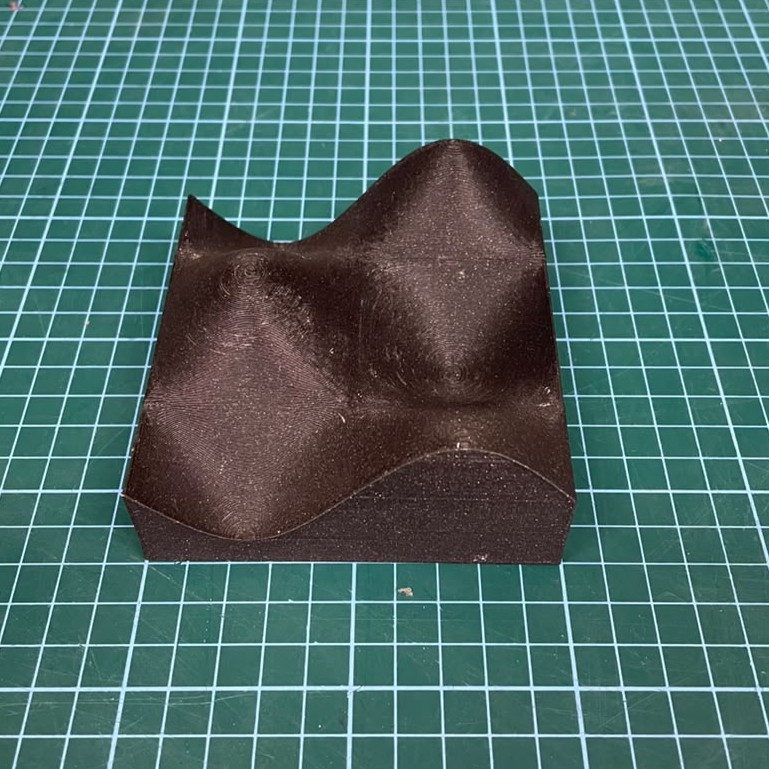
\includegraphics[width=\linewidth]{figs/Ch4/1_egg.jpeg}
        \caption{Egg carton 1}
        \label{fig:ch5.print_egg}
    \end{subfigure}
    \hfill
    \begin{subfigure}[b]{0.24\textwidth}
        \centering
        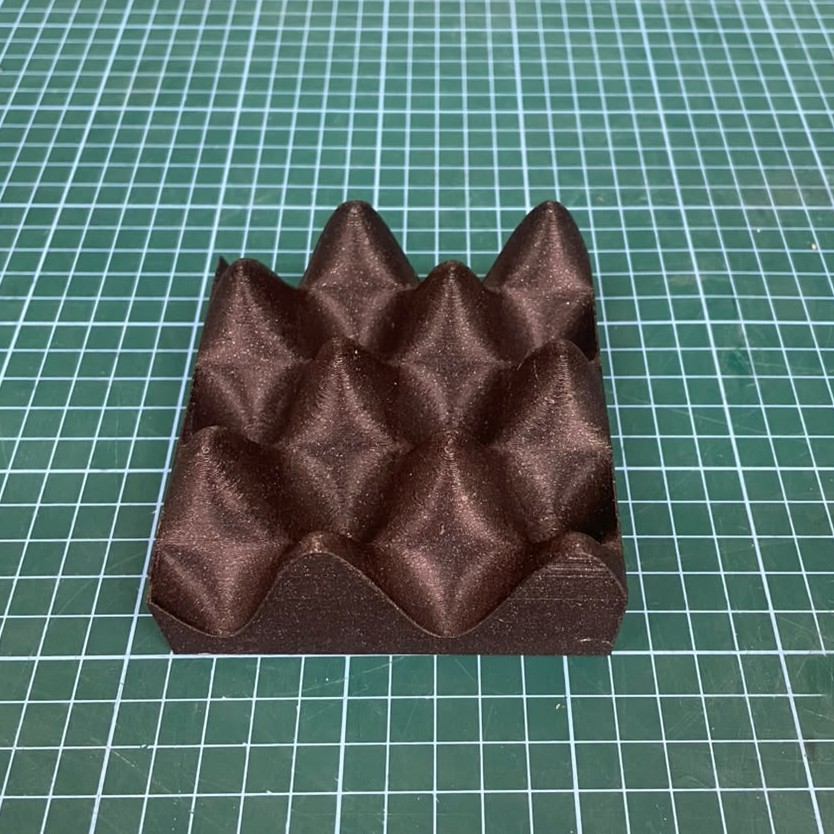
\includegraphics[width=\linewidth]{figs/Ch4/2_eg.jpeg}
        \caption{Egg carton 2}
        \label{fig:ch5.print_egg_2}
    \end{subfigure}
    \caption[3D-printed targets]{\textbf{3D-printed targets.} The four printed tiles used as
    ground truth: two pyramid tiles and two sinusoidal egg-carton tiles.}
    \label{fig:ch5.printed_shapes}
\end{figure}

\subsection{Imitation Sea Ice}
While the 3D prints are useful for measuring accuracy, they do not
represent sea ice well. The black surfaces differ from ice in both texture and contrast. 
Furthermore, under-ice scanning looks upwards towards the
surface, where incoming sunlight affects the images. To better approximate real ice, four foam structures were
cut with a hot wire and painted light blue. The set includes a grid of
2\,$\times$\,2\,cm cubes to emulate repetitive patterns, an overhang to emulate large
occlusions, a stepped pyramid to emulate layered ice, and a wave pattern to
emulate curved ice features.

\begin{figure}[htbp]
    \centering
    \begin{subfigure}[b]{0.2\textwidth}
        \centering
        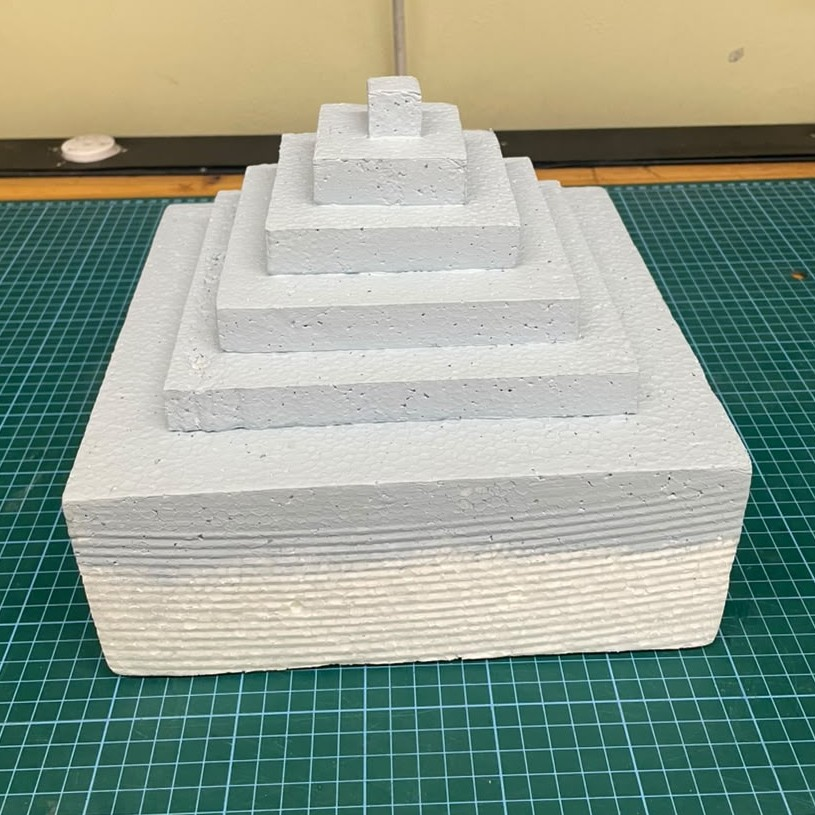
\includegraphics[width=\linewidth]{figs/Ch4/Pyr.jpeg}
        \caption{Stepped pyramid}
        \label{fig:ch5.foam_pyramid}
    \end{subfigure}
    \hfill
    \begin{subfigure}[b]{0.2\textwidth}
        \centering
        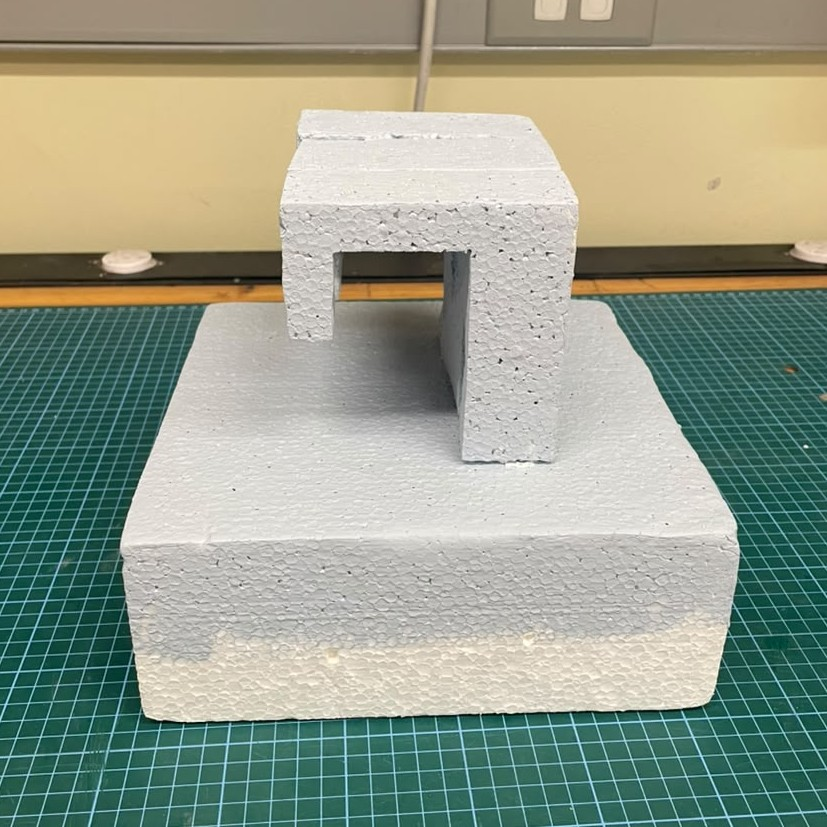
\includegraphics[width=\linewidth]{figs/Ch4/Hang.jpeg}
        \caption{Overhang}
        \label{fig:ch5.foam_overhang}
    \end{subfigure}
    \hfill
    \begin{subfigure}[b]{0.2\textwidth}
        \centering
        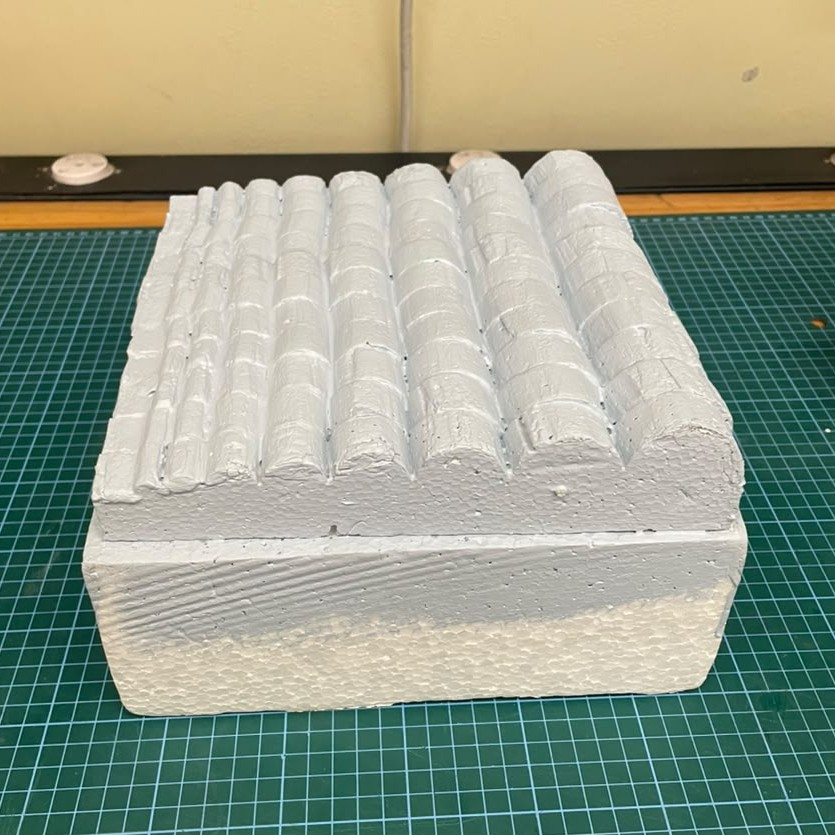
\includegraphics[width=\linewidth]{figs/Ch4/Waves.jpeg}
        \caption{Wave}
        \label{fig:ch5.foam_wave}
    \end{subfigure}
    \hfill
    \begin{subfigure}[b]{0.2\textwidth}
        \centering
        % TODO: no photo of the foam cubes yet; 2x2 pyramid print used as a stand-in
        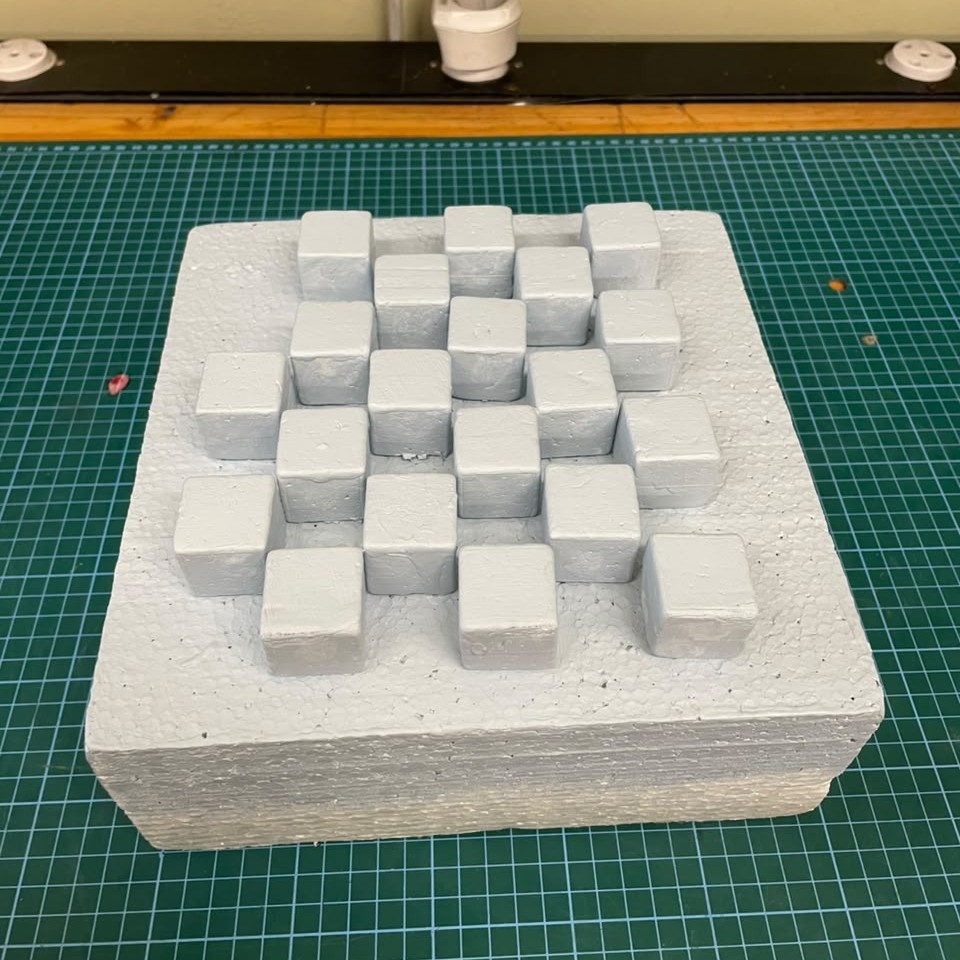
\includegraphics[width=\linewidth]{figs/Ch4/cube.jpeg}
        \caption{2\,$\times$\,2\,cm cubes}
        \label{fig:ch5.foam_cubes}
    \end{subfigure}
    \caption[Foam ice blocks]{\textbf{Foam ice blocks.} The four hot-wire-cut,
    painted foam blocks used to imitate features on the underside of sea ice.}
    \label{fig:ch5.foam_blocks}
\end{figure}

%========================
\subsection{Datasets}
\label{sec:ch4.datasets}
Data was recorded both in air, in the \gls{aru} laboratory, and water (swimming pool). The swiming pool recordings
were completed over three days, in varying lighting conditions. The time, weather and pool conditions of each recording are
explained in the GitHub repository, together with the field notes taken during recording
(\hyperref[app:gitrepo]{Appendix~\ref*{app:gitrepo}}). 

All recordings were captured in 1600\,$\times$\,1200\,px, 30\,fps, \gls{mjpeg}. The choice of \gls{mjpeg} was to allow for more than 5\,fps for 
continous capture aswell as due to an issue in setting the YUYV white balance when testing underwater. This is also the format supported by
the camera synchronisation which will aid future work.

The recordings used in this report are grouped into three datasets, DS11–DS3,
shown in \autoref{fig:ch4.datasets} and described below. 

\begin{figure}[htbp]
    \centering
    \begin{subfigure}[t]{0.32\textwidth}
        \centering
        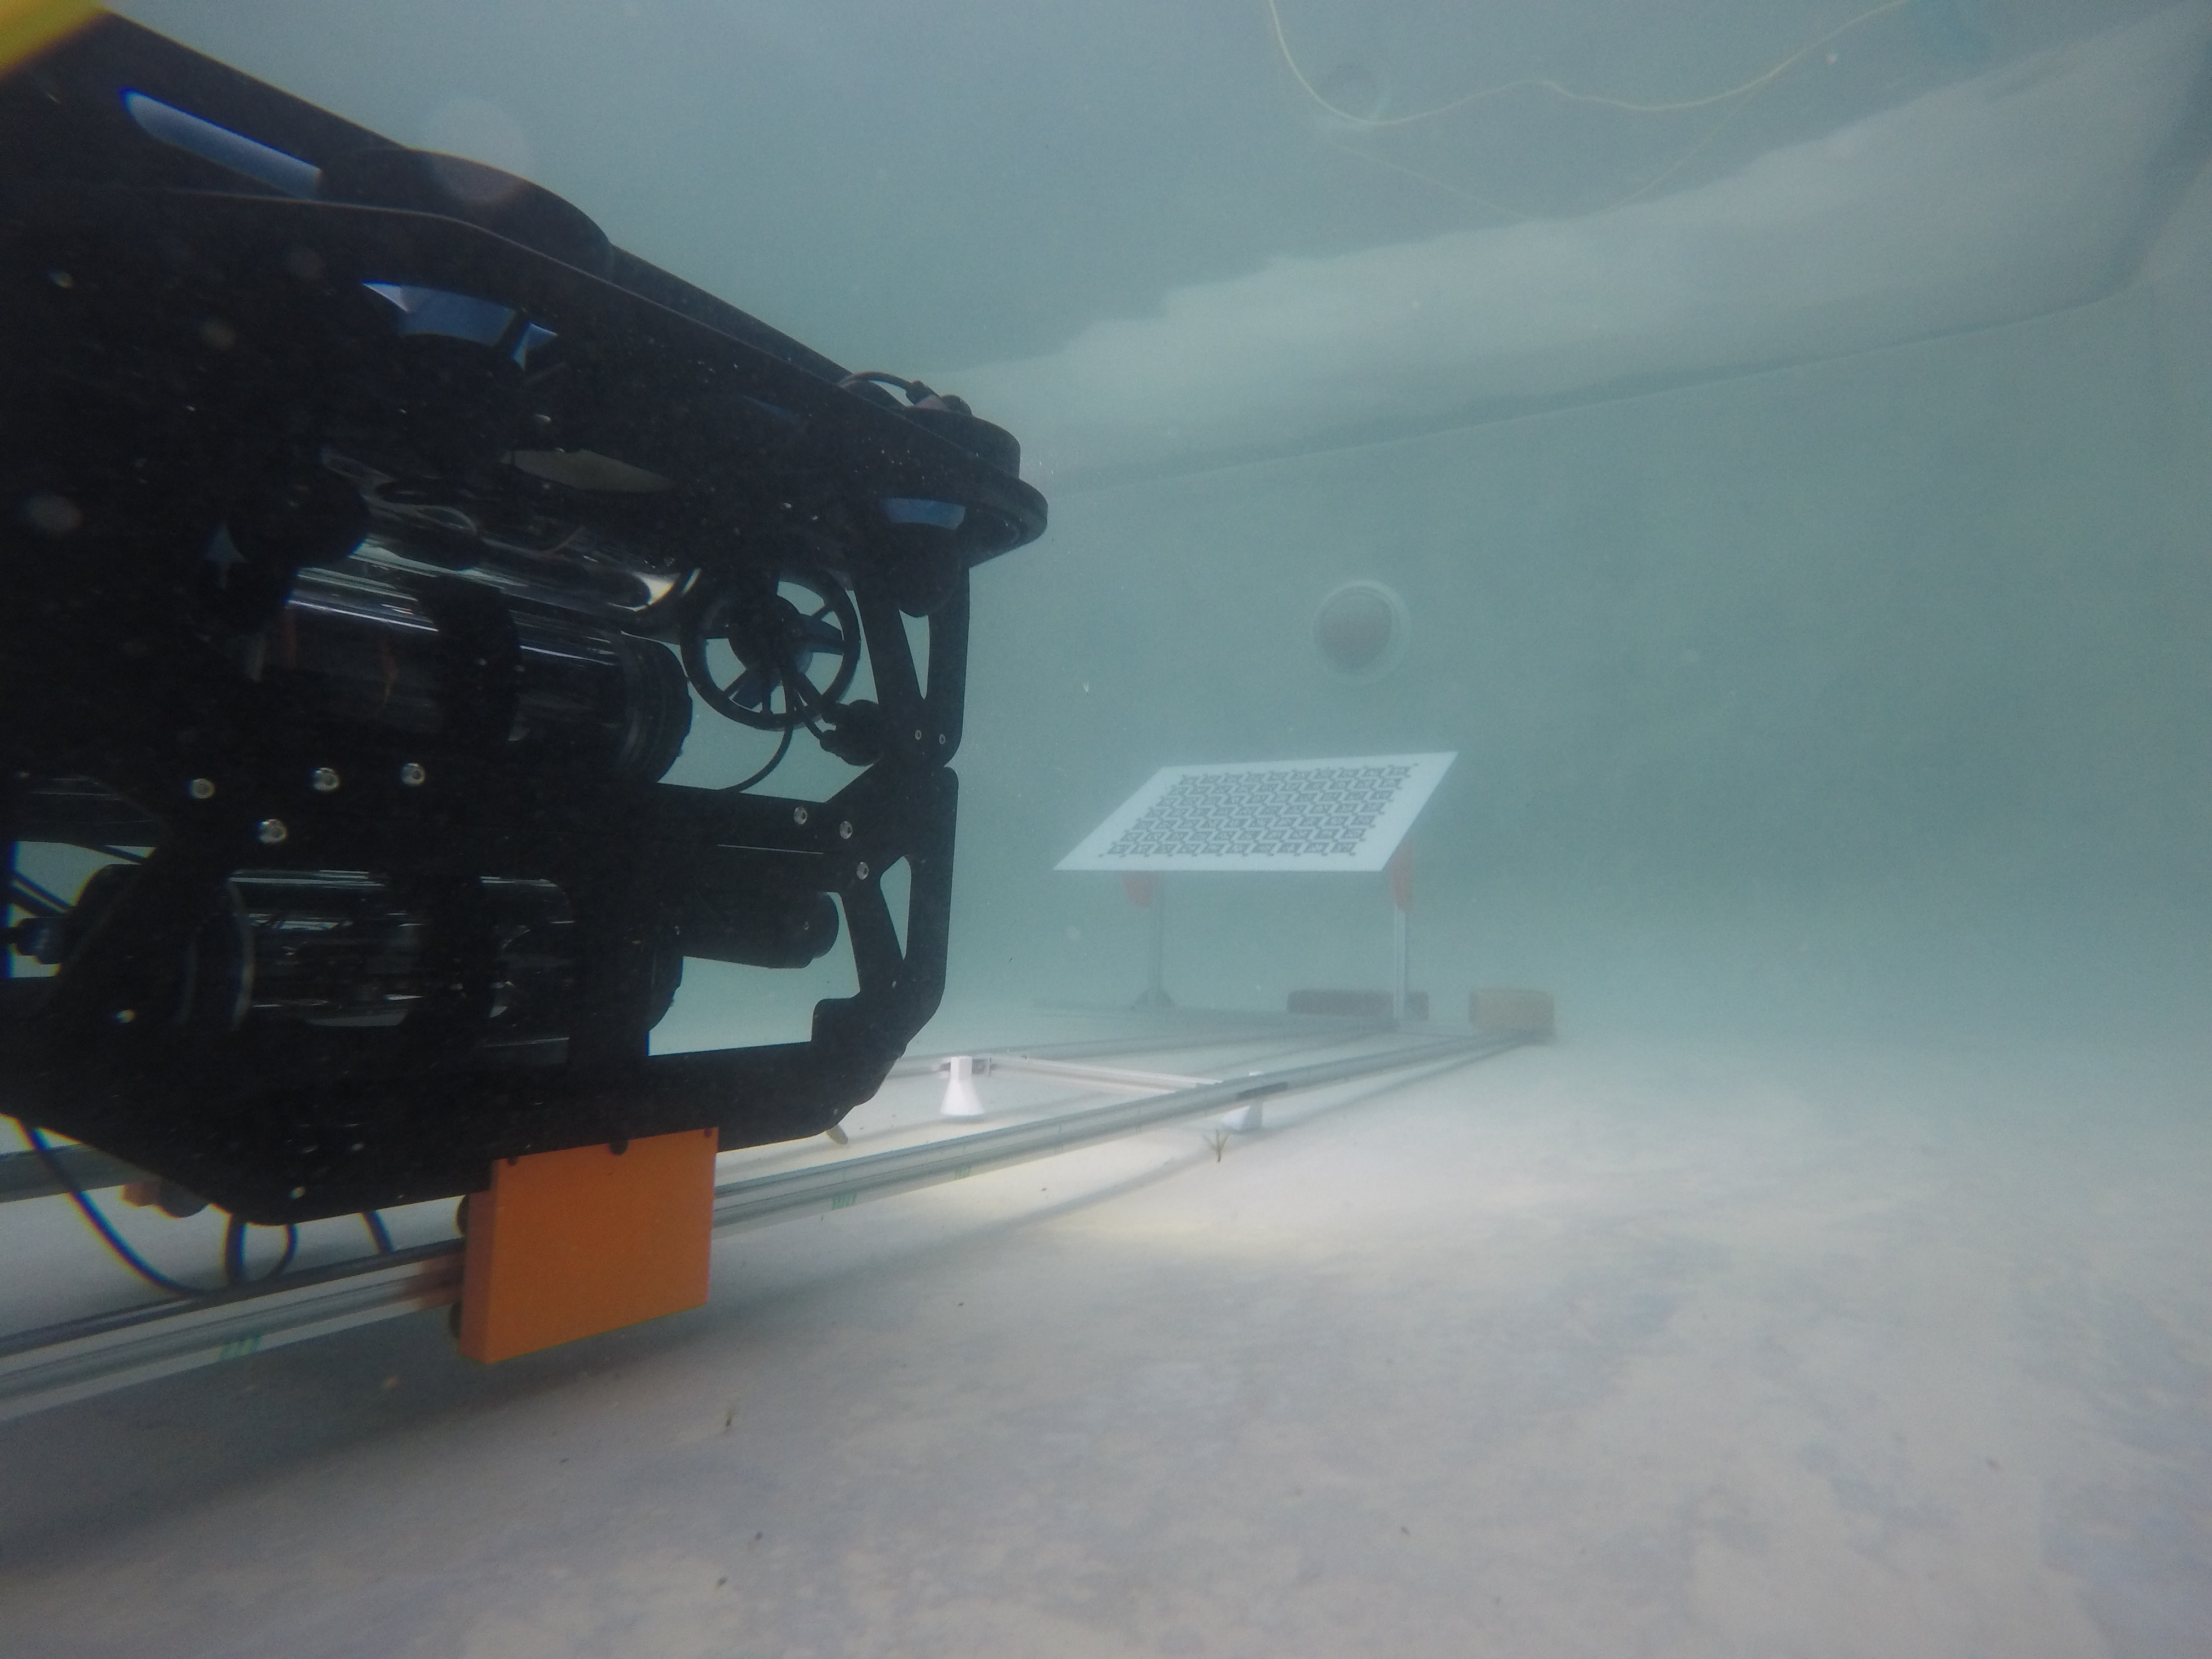
\includegraphics[width=\linewidth]{figs/Ch5/G_calib.JPG}
        \caption{DS1: calibration board at the end of the rail.}
        \label{fig:ch4.data_calib}
    \end{subfigure}
    \hfill
    \begin{subfigure}[t]{0.32\textwidth}
        \centering
        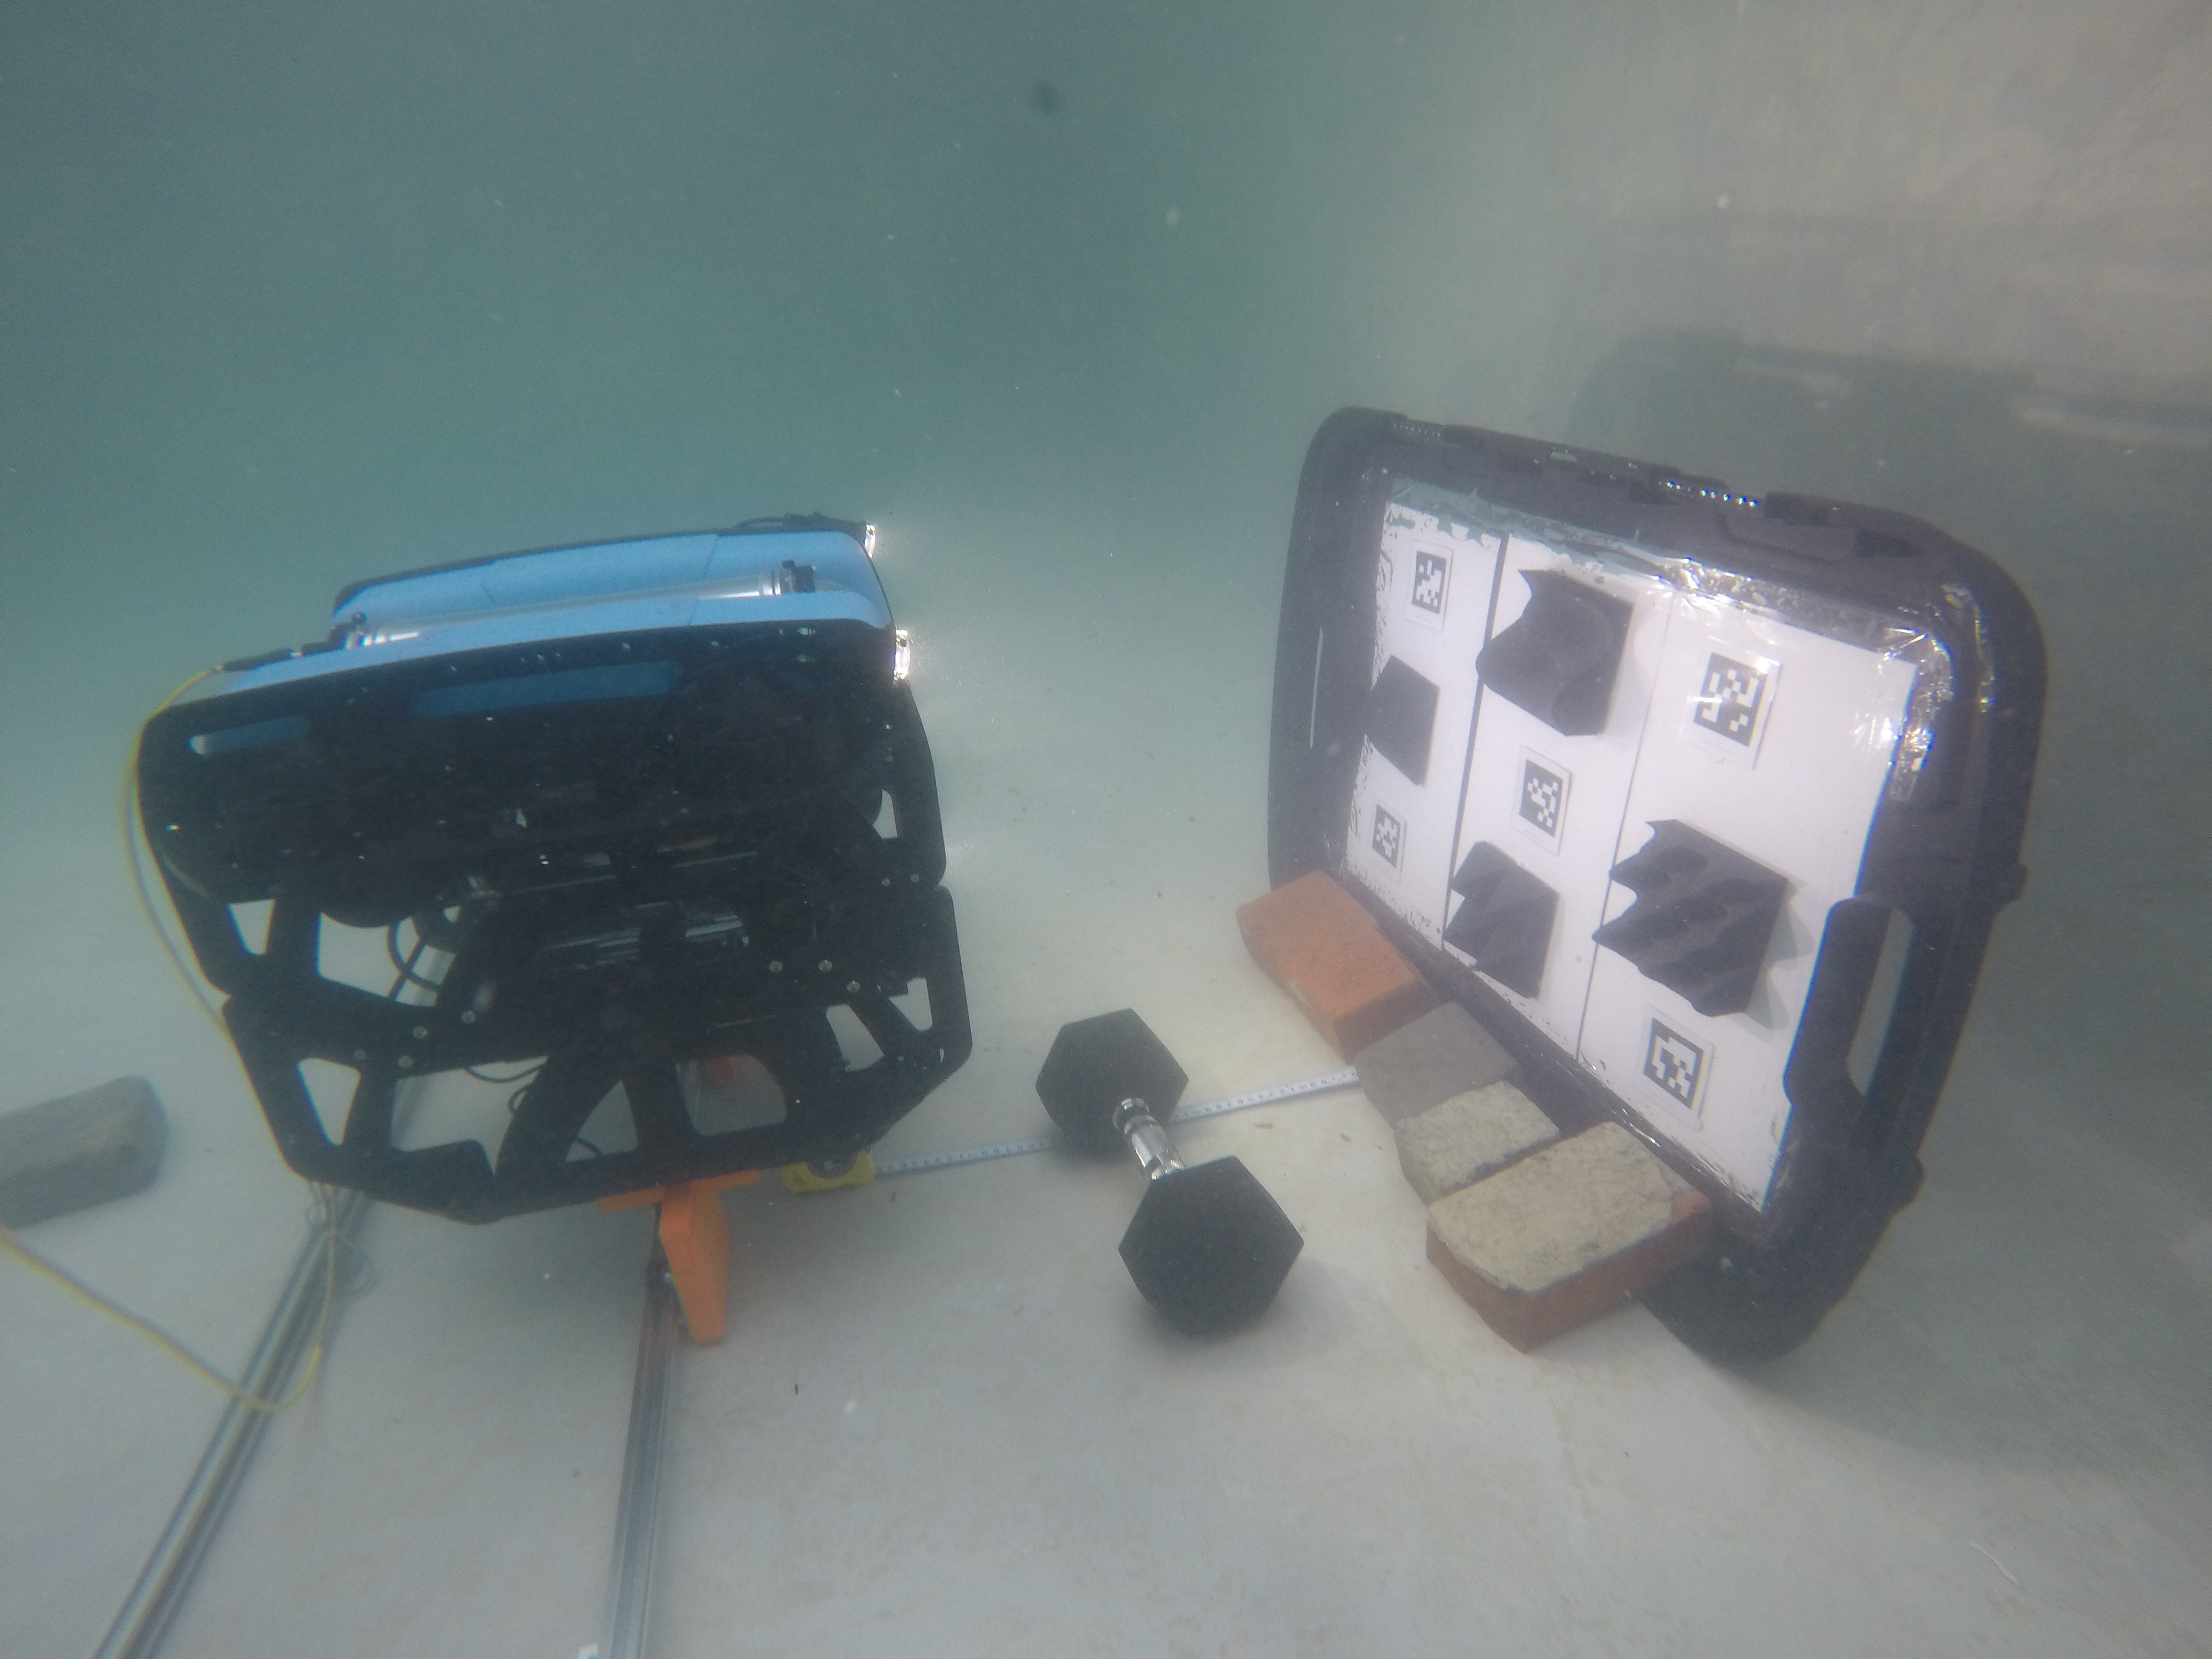
\includegraphics[width=\linewidth]{figs/Ch5/G_side.JPG}
        \caption{DS2: side scan of the 3D prints, \acrshort{rov} rotated 90\,$^\circ$.}
        \label{fig:ch4.data_side}
    \end{subfigure}
    \hfill
    \begin{subfigure}[t]{0.32\textwidth}
        \centering
        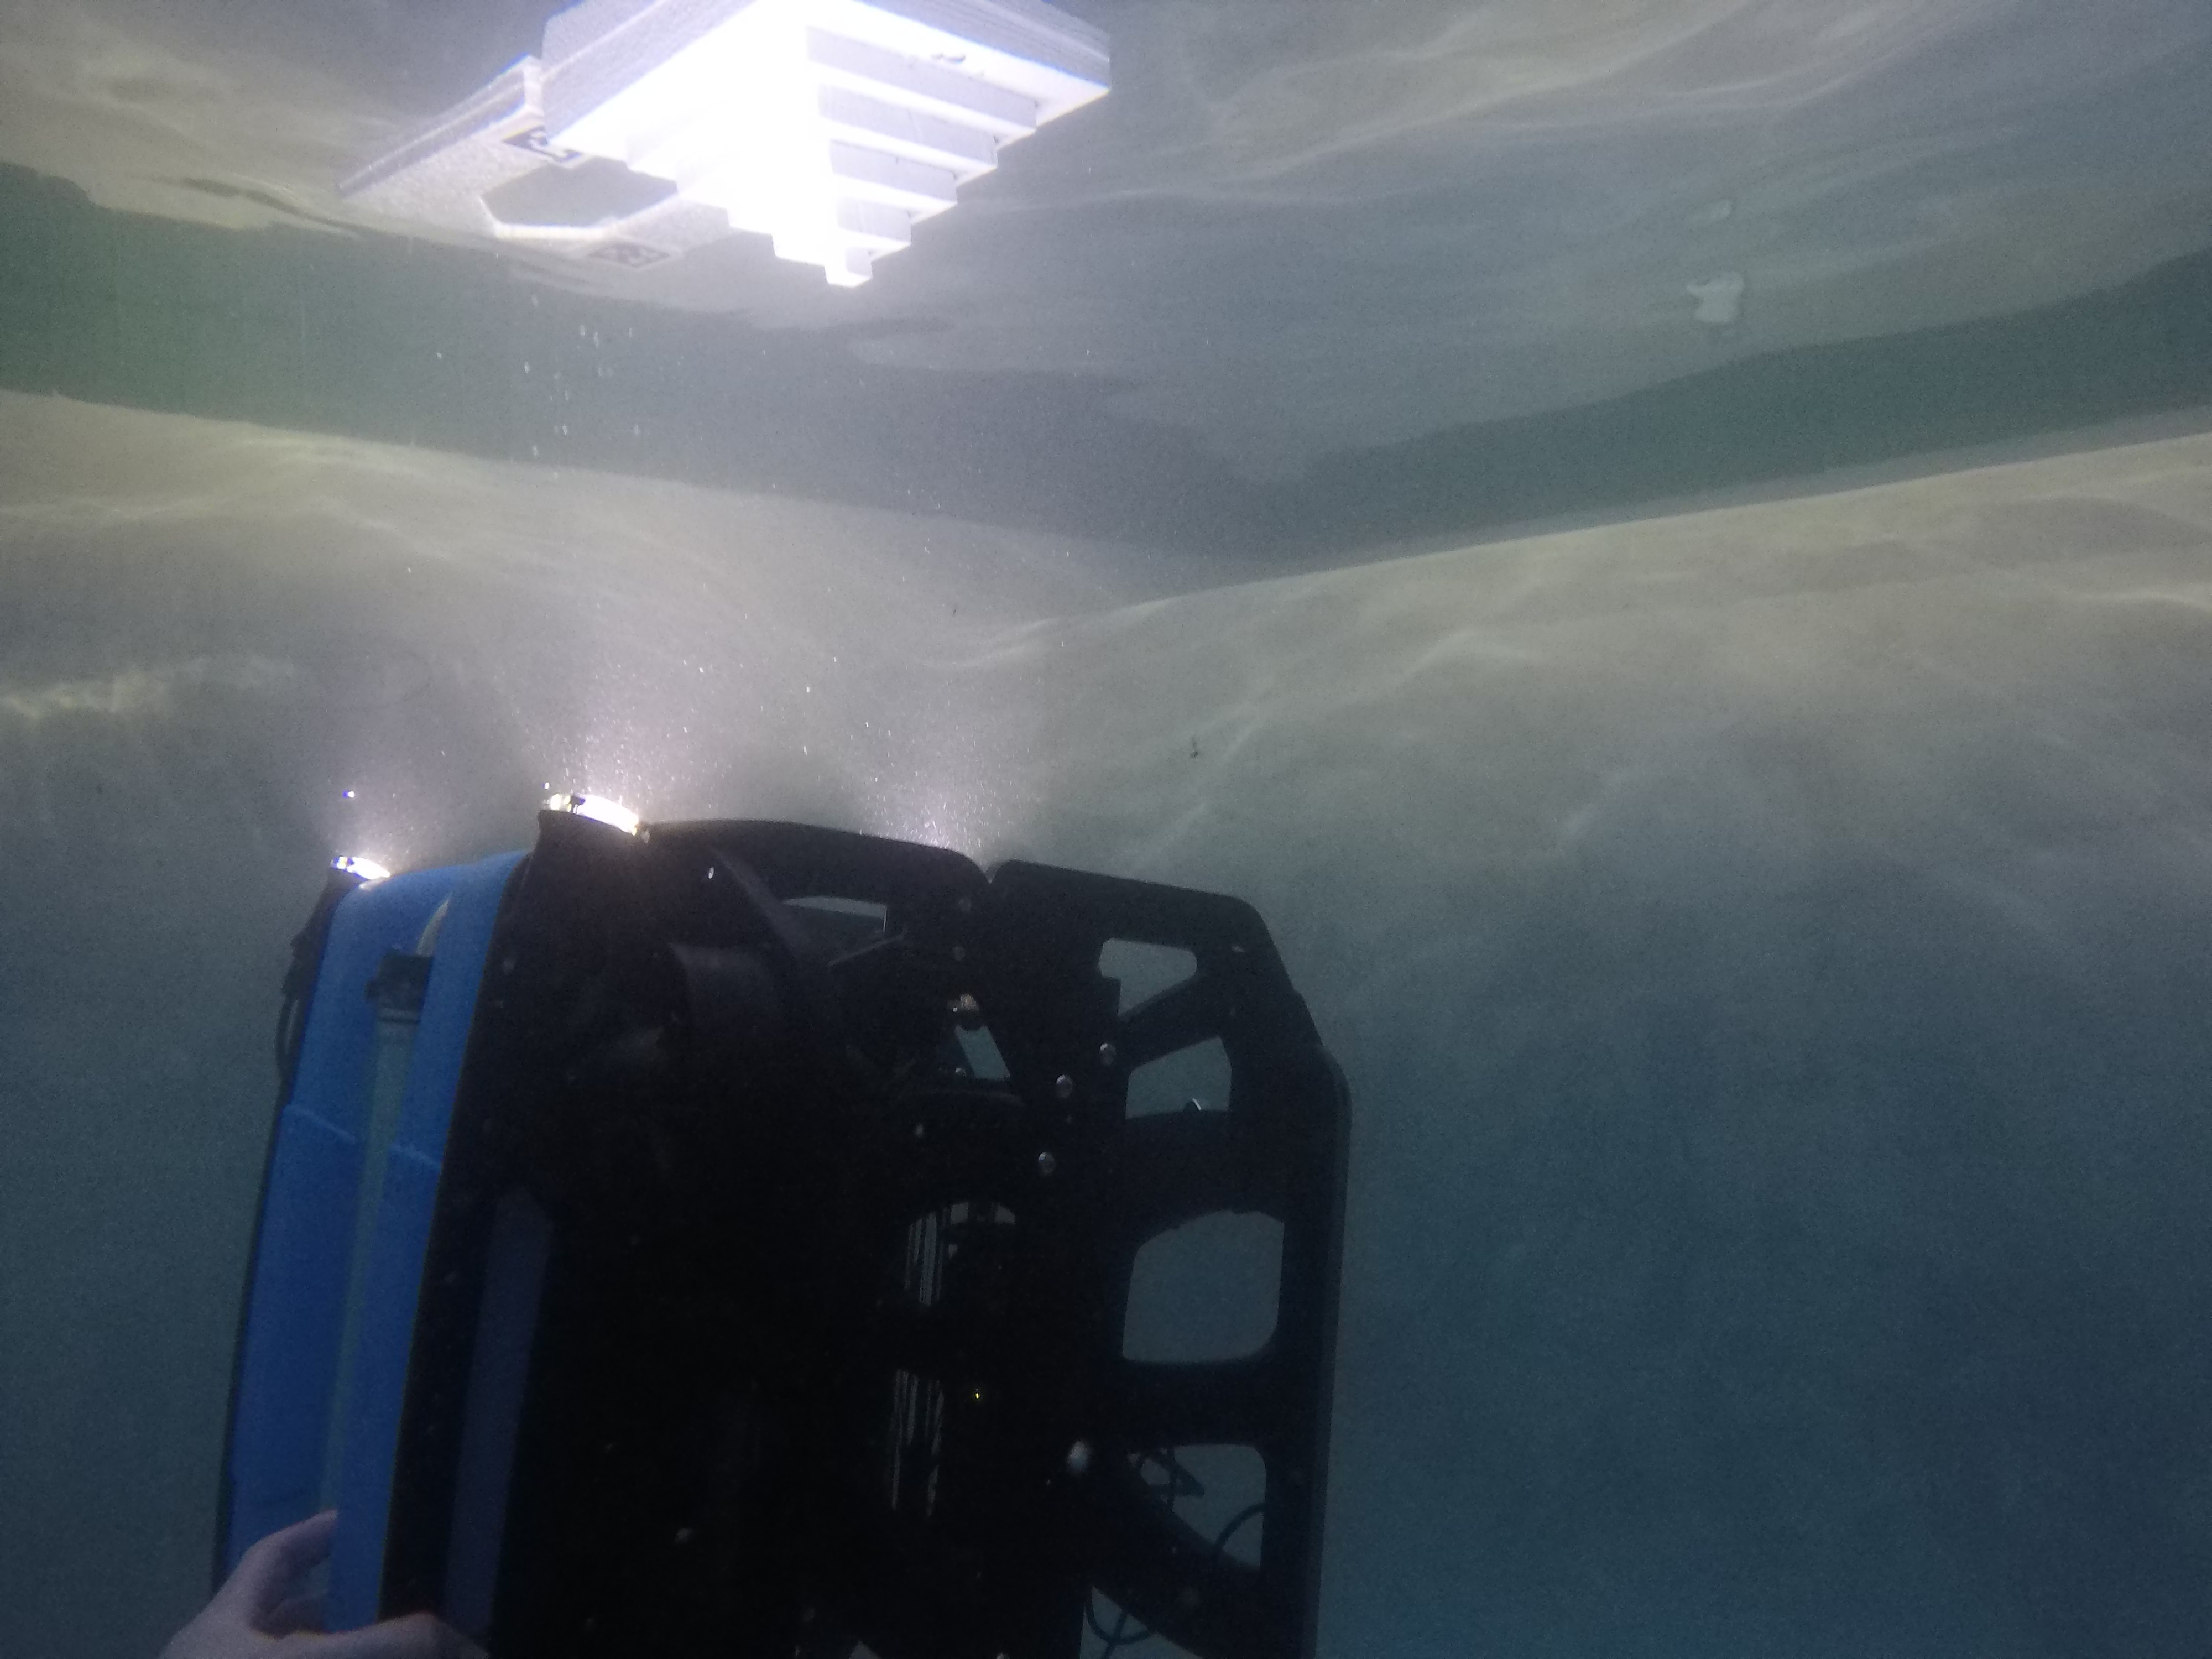
\includegraphics[width=\linewidth]{figs/Ch5/G_up.JPG}
        \caption{DS3: upward scan of the pyramid in overcast late-afternoon light.}
        \label{fig:ch4.data_up}
    \end{subfigure}
    \caption[Underwater datasets.]{\textbf{Underwater datasets.} The three datasets recorded in the pool.}
    \label{fig:ch4.datasets}
\end{figure}

%======================================
\subsubsection{DS1: Calibration Recordings}
\label{sec:ch4.ds1}
The calibration dataset was recorded on the test rail, with the calibration board mounted at one end.
The board was mounted at two positions across the rail, centre and left. Its angle, measured from the
horizontal, was set to 0, 20, 30, 40, 50 and 60\,$^\circ$ at the centre and 0, 20, 40 and 60\,$^\circ$ on the left.
At each angle, recordings were taken with the ROV for distances between 40 and 150cm at 10cm intervals.
This test was repeated both in air in the \gls{aru} experimental space, and underwater in a students pool.

\subsubsection{DS2: Side Scans of 3D-Printed Targets}
\label{sec:ch4.ds2}
The 3D-printed targets were fixed to a flat board with AprilTags placed around them. The tags provided a
ground-truth camera pose (\autoref{subsec:ch5.tag_poses}) and serve as reference points for separating the objects.
The \gls{rov} was rolled past the board, stopping every 10\,cm. This was repeated with the stereo cameras
20, 30, 40, 50 and 60\,cm from the board.

\subsubsection{DS3: Upward-Looking Scans of Foam Blocks}
\label{sec:ch4.ds3}
The four blocks were held in place in the water while a swimmer
moved the \gls{rov} around below them, with the cameras facing directly upwards.
Each block was scanned separately, next to a flat foam block carrying AprilTags. As in DS2, the tags
provide a ground-truth reference. Each scan consists of a single pass. Due to the fact that the \gls{rov} was not fixed
in place, the distance to the blocks was found by triangulating the AprilTags.

The scans were repeated in two conditions. The first set were in direct sunlight at around 13:00, and again in overcast
late-afternoon light at around 17:00. \autoref{fig:ch4.data_up} shows a scan of the pyramid in the
darker conditions.
